\subsection{DDI with SVM}

The third implementation trains a Support Vector Machine model to perform Drug-Drug interaction detection and classification for each drug pair appearing in each sentence. All code is based on Python 3 and Scikit-learn. As before it uses modules for interacting with Freeling, perform the lookup of words on a DrugBank lookup and the like. This time, the model feature matrix input will contain features from words in the sentence, and features extracted from the sentence.

\textbf{Features}

%The complete set of features prepared for this model is the same used in the previous smv model (this time only applied to each drug of the pair), but adding features from the context of the sentence.

For the second task to detect drug drug interactions, we have used the single word features for each entity word  \ref{table:DNRfeatures} (in the pair) also with a context window of 3. Then we have added the features derived from the dependency tree (appearances of frequent trigrams, words, lemma, pos. We also added counts of specific POS tags (verbs , determiners, etc).

\begin{table}[H]
\centering
\begin{tabular}{lll}
\multicolumn{3}{l}{Drug-Drug Interaction Features}                                       \\ \hline

$f_{1}$ & All DNR SVM features        & for each entity of the pair   \\
\rowcolor[HTML]{DAE8FC} 
$f_{2}$ & All DNR SVM features in a window        & \begin{tabular}[c]{@{}l@{}}for each word  \\ in a window 0 to 5 \end{tabular}                      \\
$f_{3}$ & Appearance of most frequent 3-gram sequences & from dependency tree shortest path    \\
\rowcolor[HTML]{DAE8FC} 
$f_{4}$ &  Appearance of most frequent Word/Lemma  &        \\
$f_{5}$  & Appearance of most frequent POS  & from CFG parse tree shortest path    \\
\rowcolor[HTML]{DAE8FC} 
$f_{6}$ &  Word count in the shortest path  & from dependency tree shortest path        \\
$f_{7}$ &  Counts of POS tags in sentence   &  specific tags: VB, CC, MD, DT

\end{tabular}
\caption{DDI features}
\label{table:DDIfeatures}
\end{table}




For the Word embedding feature, we used pre-processed database from Pubmed$^{\cite{PubMedDatabase}}$, that contains a Word2Vec model with a 200 words context size. We were'nt able to use this feature due to memory limitation (200 float values per word).\\
For the contextual features, used in the drug drug interaction task, we created different parse trees (Dependency and CFG). In figure \ref{fig:deptree}  we have an example of a dependency tree in a sentence with 2 drugs . We extract the shortest path from the parse tree for each pair interaction and sentence. Then for each shortest path we extract the trigrams, words, lemma , pos and we count how many times each of them appears in the whole training data set. Finally we keep the more frequent ones with a specific threshold (50 for memory size reasons). And finally the feature for each pair- sentence will be the binary var that indicates each of the frequent words/trigrams/etc is in the sentence's shortest path or not.

\textbf{Feature vector}

The SVM model for DDI is trained on a sentence feature vector basis. This includes all the possible features of each drug word in a pair and the words in a context window of 0 to 5, plus the sentence features which are appearances of frequent trigrams, words, lemmas and postags from the dependency tree, as well as counts of POS tags and words. The structure of the feature vector for each word is shown in the figure \ref{fig:ddisvm}.




\begin{figure}[H]
\minipage{0.5\textwidth}%
  \centering
  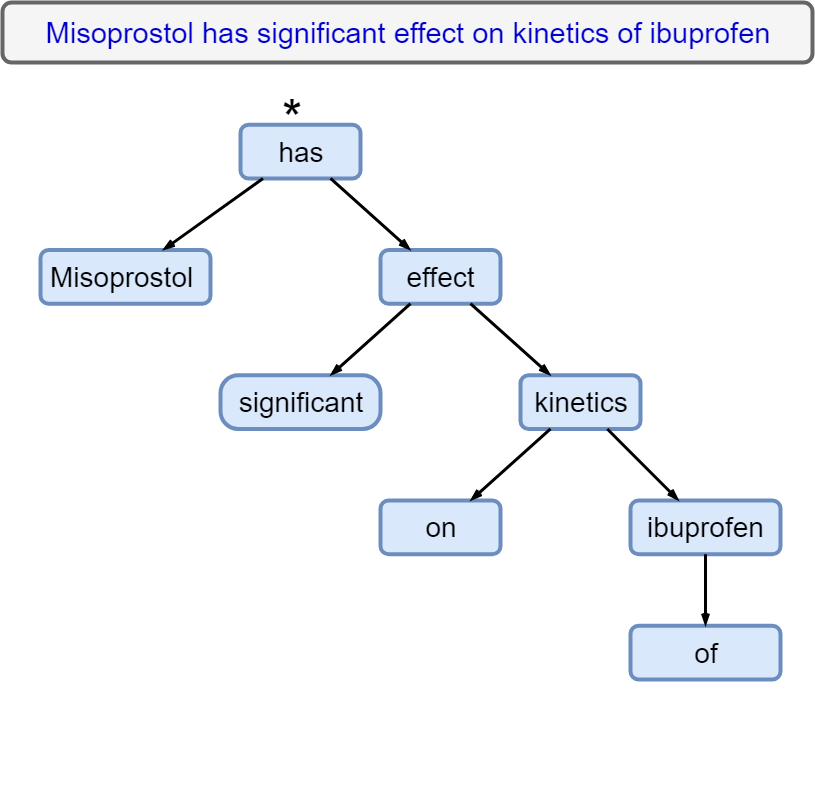
\includegraphics[scale=0.25]{tree.png}
  \caption{Dependency tree }\label{fig:deptree}
\endminipage\hfill
\minipage{0.5\textwidth}
    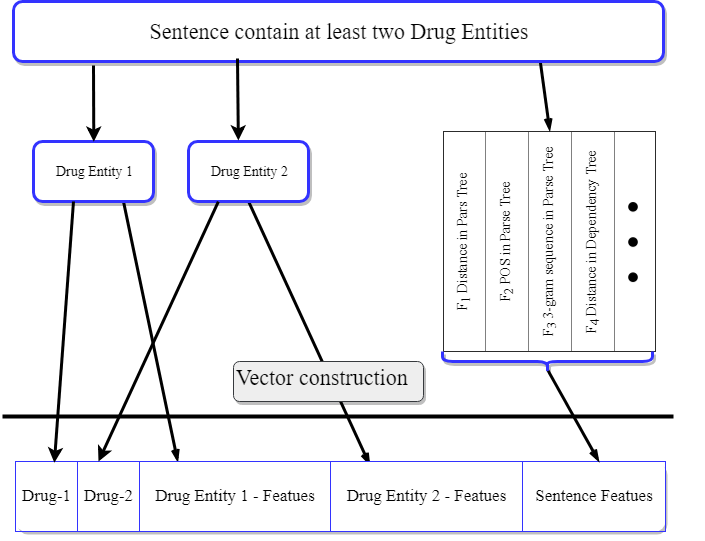
\includegraphics[width=\linewidth]{DDI.png}
  \caption{Feature vector for DDI task}\label{fig:ddisvm}
\endminipage
\end{figure}












